\chapter{Lecture 15 - Lighting}
Lighting can be perceived and mathematically modeled in different ways:
\begin{itemize}[noitemsep]
    \item \textit{Ray optics}: the light is modeled using rays. The rays follow geometric rules, which can model several lighting effects like reflection and refraction
    \item \textit{Wave optics}: the light is modeled as a propagating wave, which can model lighting effects such as diffraction
    \item \textit{Electromagnetic optics}: it can describe lighting effects like the polarization of the light, not explained by the wave optics
    \item \textit{Photon optics}: quantum mechanics is used to model lighting effects
\end{itemize}

The lighting is a process where energy is emitted from a source (like a lamp or the sun), travels through a scene, and interacts with objects until it stabilizes. This happened at the speed of light, making the result appear instantaneous and table to the human eye.\par
When a ray of light hits a surface, several effects happen simultaneously: specular reflection (light bounced off in a specific direction, like a mirror), diffusion (light scatters in many directions), transmission (light passes through the material, refraction), absorption (the material soaks up the energy), and scattering/emission (effects like fluorescence).

\subsubsection{Solid angle}
To calculate lighting in 3D space, the solid angle (\(\Omega\)) is introduced, which is the 3D extension of a 2D planar angle. It represents the angular dimension of a cone pointing in a specific direction. It is measured in steradians (sr). A full hemisphere corresponds to a solid angle of \(2\pi\) steradians.

\begin{figure}[htbp]
    \centering
    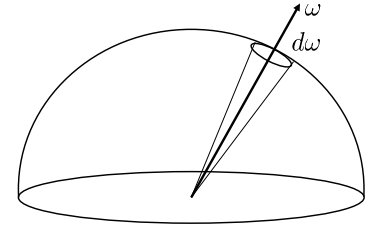
\includegraphics[width=0.3\linewidth]{imgs/lecture15/15.1 solid angle.png}
    \caption{Solid angle}
    \label{fig:15.1}
\end{figure}

\subsubsection{Radiometry}
Radiometry defines three critical units used to quantify light in a scene:
\begin{itemize}[noitemsep]
    \item Radiant flux \(\Phi\), measured in Watts, this is the total radiant energy passing through a surface per unit of time
    \item Irradiance \(E\), the radiant flux incident on a specific surface element (\(Watts/m^2\))
    \item Radiance \(L\), the radiant flux per solid angle per unit area (\(Watts/m^2sr\)). This is effectively what a camera or an eye "sees" from a specific direction
\end{itemize}

A fundamental takeaway is that for a point light source emitting light uniformly in all directions, \textit{the intensity (irradiance) reduces with the square of distance} (\(1/r^2\)).

\section{Rendering equation}
\begin{definition}[Rendering equation]
    The rendering equation is the fundamental formula for calculating the total visible light (\(L_o\)) at any point on a surface from a specific direction. 
\end{definition}

The rendering equations calculate the visible light in a point of the scene for a specific direction, given by the sum of emitted light and the light reflected in that direction: \textit{emitted light} (\(L_e\)), which is the energy the object produces itself; and \textit{reflected light} (\(L_r\)), which is the light from the environment that bounces off the surface. To find the reflected light, the algorithm must integrate all incoming light contributions from every direction in the hemisphere above the point, weighting them according to the material's properties and the angle of reflection.\par
There are two specialized functions to mathematically represent how different surfaces (wood, metal, skin ..) look; these two are BSSRDF and BRDF

\subsubsection{BSSRDF}
Bidirectional Scattering Surface Reflectance Distribution Function.\par
The function describes the most general case of light-material interaction, where light hits a surface and may leave from a different position; the process is called scattering.

\subsubsection{BRDF}
Bidirectional Reflectance Distribution Function.\par
Because of the complexity of BSSRDF, computer graphics often uses the BRDF as an approximation. It assumes light enters and leaves at the same point x. It is defined as the ratio between the outgoing radiance (reflected light) in a certain direction and the incident irradiance (incoming light) from another direction.

\section{Local lighting model}
Because calculating the full rendering equation is computationally too expensive for real-time systems, designers use local lighting models to approximate the way light interacts with surfaces. These models focus only on the local effects, ignoring the complex "global" inter-reflection between all objects in a scene.

\begin{definition}[Global effects]
    Global effects involve interactions between multiple objects, such as soft shadow, indirect lighting (color bleeding), and caustics
\end{definition}

\begin{definition}[Local effects]
    Local lighting models simplify the scene by calculating light for a single point based only on its own properties and the direct light sources, ignoring reflections from other objects.
\end{definition}

\subsection{Phong lighting model}
The Phong model is a fundamental tool for simulating how \textit{opaque} materials look under a point light source. While it is quite realistic, the sources note that some materials can end up looking like plastic. It simplifies the math by breaking the final color into three distinct components:
\begin{itemize}[noitemsep]
    \item \textbf{Ambient component}: this term is used to \textit{roughly approximate global inter-reflections}. It provides a constant base level of light to all points in the scene so that areas not directly hit by a light source are not completely black
    \item \textbf{Diffuse components}: based on Lambert's law, this represents \textit{light that hits a rough surface} (like wood or stone) and reflects uniformly in all directions. The intensity depends on the angle (\(\theta\)) between the light source and the surface normal; it is brightest when the light is directly overhead
    \item \textbf{Specular component}: this models the "shiny" part of an object, the specular highlight. It \textit{simulates light reflection off smooth, mirror-like surfaces} in a specific direction. Unlike diffuse light, the appearance of the specular highlight depends on the position of the observer.
\end{itemize}

A critical part of the specular term is the exponent (n). This parameter defines how "sharp" or "focused" the specular highlight is. A high value of n creates a very small, bright portion of light (like a polished billiard ball), while a lower value makes the highlight larger and more spread out.\par
The model also accounts for light attenuation, where the intensity of the light source decreases as the distance (\(d_L\)) from the light to the surface increases.

\section{Shading}
\begin{definition}
    Shading is the process of computing the actual color of each pixel on the screen based on the lighting models. It determines where and how often the light-material interactions are calculated on a 3D model
\end{definition}
There are three primary types of shading: Flat shading, Gouraud shading, and Phong shading.

\subsubsection{Flat shading}
Flat shading is the simplest form of shading, where the lighting equation is computed only once for each face (polygon) of the 3D model. In which the algorithm uses the face normal to determine a single color, which is then applied uniformly across the entire surface of that face. \par
Because each face has a single solid color, the edges between them become very obvious, and the object looks "blocky." Even if you use a massive number of faces to try to smooth the object, it will fail to smooth the edges.

\begin{figure}[htbp]
    \centering
    \includegraphics[width=0.5\linewidth]{imgs/lecture15/15.2  flat shading.png}
    \caption{On the left, the flat shading, on the right, the reference object}
    \label{fig:15.2}
\end{figure}

The visual effect of \textbf{Mach Banding} is the perceptual phenomenon where the human eye exaggerates the contrast at the borders between different shades, making discontinuities clearly visible, thus explaining the presence of "blocky" edges.

\begin{figure}[htbp]
    \centering
    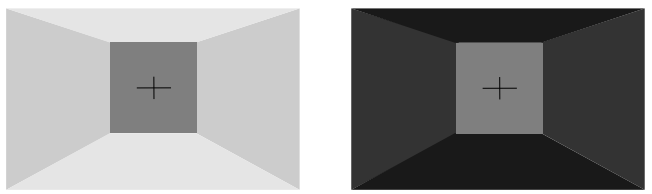
\includegraphics[width=0.5\linewidth]{imgs/lecture15/15.3 mach banding.png}
    \caption{Mach Banding}
    \label{fig:15.3}
\end{figure}

\subsection{Gouraud shading}
To fix the blockiness of flat shading, Gouraud shading calculates the lighting at the vertices instead of the faces. The lighting equation is computed for each vertex using a vertex normal (often calculated as the average of the normals of the faces meeting at that vertex). The colors at the vertices are then linearly interpolated across the face of the triangle during rasterization. This creates a much smoother appearance, making faceted models look like continuous curved surfaces.\par
But, it struggles with specular highlights. If a highlight (the bright, shiny spot) falls in the middle of a face rather than near the vertex, it might be missed entirely or appear distorted because the interpolation only knows about the colors at the corners. It can also have visual issues at the corners of objects.

\subsection{Phong shading}
Phong shading provides the highest quality results by moving the lighting calculation from the vertices to the individual pixels (fragments). Instead of interpolating the colors from the vertices, this method interpolates the surface normals across the face of the triangle. The lighting equation is then computed for every single pixel using these interpolated normals.\par
This is the most realistic method out of the three. It correctly renders specular highlights even if they are very small or fall in the center of a face, and it provides a perfectly smooth appearance for curved surfaces.

\begin{figure}[htbp]
    \centering
    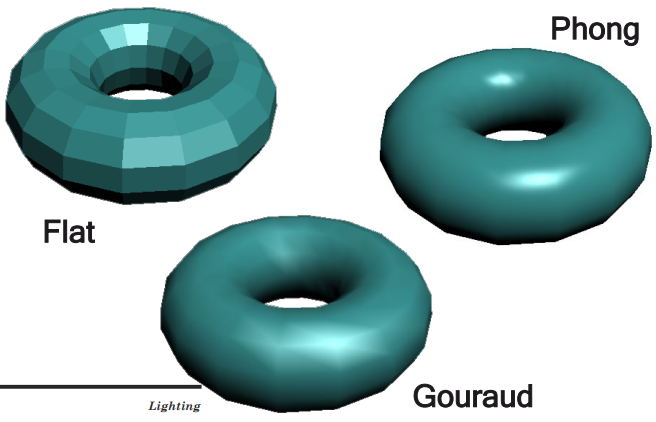
\includegraphics[width=0.5\linewidth]{imgs/lecture15/15.4 shading.png}
    \caption{Shading methods result comparison}
    \label{fig:15.4}
\end{figure}